\documentclass{beamer}
\usepackage{tabularx}
\usepackage{multicol}
\usetheme{Copenhagen}

\newcommand{\logit}{\mathrm{logit}}

%\AtBeginSubsection[]{
%  \begin{frame}
%  \vfill
%  \centering
%  \begin{beamercolorbox}[sep=8pt,center,shadow=true,rounded=true]{title}
%    \usebeamerfont{title}\insertsectionhead: \insertsubsectionhead\par%
%  \end{beamercolorbox}
%  \vfill
%  \end{frame}
%}

\AtBeginSubsection[]
{
    \begin{frame}{Outline}
      \small
      \begin{multicols}{2}
      \tableofcontents[currentsection,currentsubsection]
      \end{multicols}
      \normalsize
    \end{frame}
}


\title[]{An Intelligent Tutoring System Utilizing Bloom's Taxonomy and
Item-Response Theoretic Assessment}
\author{Dennis Castleberry}
\date{\today}

\begin{document}

\frame{\titlepage}


\frame{ \frametitle{Contents}
      \small
      \begin{multicols}{2}
      \tableofcontents
      \end{multicols}
      \normalsize
}


\section{Preliminaries}

\subsection{Introduction}


\frame{ \frametitle{Motivation}
  \begin{itemize} 

    \item Students have variance in \textbf{trait ability}, that is internalized
    problem-solving ability, with respect to certain skills.  
    
    \item Targetting any segment of the distribution of students provides that
    segment with attention at the expense of other segments.  

  \end{itemize} 
}



\frame{ \frametitle{Motivation}

  \begin{itemize} 

    \item In addition, students may have different levels of ability with
    respect to different skills, and may have different interests as well.

    \item We would like to personalize teaching, but accommodating each student
    individually with a classical approach is prohibitively time-consuming.

    \item Thus we introduce ITS ({intelligent tutoring systems}) to help
    us.

  \end{itemize} 

}



\frame{ \frametitle{ITSs and CATs}

  \begin{itemize} 

    \item A \textbf{Computer Adaptive Tester}, or CAT, is a system which
    assesses a student adaptively, basedon the student's prior responses. 

    \item An \textbf{Intelligent Tutoring System}, or ITS, is a system which
    aims to raise a student's ability.

    \item An ITS may contain a CAT, but the goal is different.

  \end{itemize} 

}


\frame{ \frametitle{CATs}

  Three main advantages of CATs:  

  \begin{itemize} 

    \item They easily lend themselves to \textbf{formative testing}, which is
    beneficial for students \cite{bull2003blueprint} \cite{mead1993equivalence}
    \cite{bangert1991instructional} \cite{lawton2012online};

    \item They are amenable to the {scientific exploration of learning
    theories}, since data is highly available and \textbf{testing algorithms}
    are easy to implement \cite{mayer2002multimedia}
    \cite{wainer2000computerized};

    \item They allow for the implementation of algorithms to determine the
    series of questions to be asked, allowing for \textbf{dynamic testing};
    they can even be used for curriculum sequencing
    \cite{chen2006personalized}.

  \end{itemize} 

}


\frame{ \frametitle{How CATs Work}
  Typical workflow \cite{veldkamp2013bayesian}:
  \begin{enumerate} 
    \item initial ability estimate, 
    \item selection and administer item,
    \item update ability estimate, 
    \item finally, check stopping criterion.
  \end{enumerate} 
}



\frame{ \frametitle{Types of ITSs}
  Two ways of categorizing the general approach for ITS:
  \begin{itemize} 
    \item Deficit assessment vs. error analysis \cite{bejar1984educational}
    \item Characterization-based vs process-based \cite{anderson1996act}
  \end{itemize} 
  The present ITS would be characterization-based, and utilize
  deficit assessment.
}



\frame{ \frametitle{The State-of-the-Art}
  \begin{itemize} 
    \item John Anderson's ACT-R models qualify as the most comprehensive
    and best-known basis for ITS.

    \item Anderson's ITS is process-based (mimics logic programming in
    that it has goals, facts, and rules).  Attempts to model every step
    in the process.

    \item The problem with Anderson's is that it is so fine-grained, that it is
    prohibitively time-consuming to apply to a whole course.
  \end{itemize} 
}



\frame{ \frametitle{Objective}
  Any educational program can be thought of as a sequence of tuples
   \[
     (\chi_i, t_i)
   \]
  which is an item scheduled at a time. An item could be a question or an
  informative content item. When placed in sequence, these form a schedule:
   \[
     X = \langle (\chi_1, t_1), (\chi_2, t_2), \ldots (\chi_n, t_n) \rangle.
   \]
  The present work seeks to answer the question: knowing the properties of
  these items, and having per-student information about the responses to
  these items at any point $i$, how should the remainder of the items be
  sequenced (or scheduled)?
}



\frame{ \frametitle{Novel Contributions}

  \begin{itemize} 

   \item The graph data structure to represent an assessment, whose nodes are
   items, and whose edges represent dependencies;

   \item A modification to an existing assessment theory known as Item Response
   Theory, which now accounts for dependency relationships;
   
   \item A scheduler, or algorithm whose purpose was to determine what the
   questions should be given the item parameters and the students' response
   sets;

   \item An addendum to an existing theory of memory, forgetting, and practice,
   which could then be integrated into the scheduler to provide a
   fuller-featured system.

  \end{itemize} 

}



\subsection{Background}



\frame{ \frametitle{Bloom's Taxonomy}

  \small
  \begin{itemize} 

    \item \textbf{Knowledge}. Recalling factual information.  \emph{What is a
    for-loop?}

    \item \textbf{Comprehension}. Assigning meaning to information.  \emph{What
    does the example for-loop output? (Give example.)}

    \item \textbf{Application}. Applying a rule to a specific instance.
    \emph{How can the update statement of the loop be changed to print only
    even numbers?}

    \item \textbf{Analysis}. Breaking information into parts and exploring
    relationships.  \emph{What would happen if the update statement decremented
    instead of incremented the counter?}

    \item \textbf{Evaluation}. Judging the use of knowledge or the validity of
    an argument.  \emph{Which is better for reading user input: a for-loop or a
    while-loop? Why?}

    \item \textbf{Synthesis}. Utilizing knowledge to create a new solution to
    satisfy a goal.  \emph{Write a for-loop to print only even numbers up to
    ten.}

  \end{itemize} 
  \normalsize

}



\frame{ \frametitle{ITS and Bloom}
  \begin{itemize} 

    \item Some systems incorporating Bloom levels exist, with the intent of
    supporting finer-grained characterization-based models
    \cite{sitthisak2007towards}.

    \item Such systems tend to treat Bloom levels like difficulty levels
    \cite{raykova2011adaptive}.

    \item Specialized systems (e.g. for biological sciences) use Bloom's
    taxonomy for questioning at higher levels \cite{ccepni2006effects}
    \cite{hopson2001using}.

  \end{itemize} 
}



\frame{ \frametitle{MCQs and Bloom}

  \begin{itemize} 

    \item The subjectivity of reasoning at high levels is at odds with the
    closed-ended nature of MCQs.

    \item Even for the Evaluation level, it is possible to design MCQs which
    raters agree have a definite correct/incorrect response
    \cite{lemons2013questions}.  

    \item CATs developed for use in the biological sciences have demonstrated
    that MCQs can be adapted to the higher Bloom levels
    \cite{hernan2008testing}, \cite{lemons2013questions}.  E.g. diagnoses given
    symptoms (Evaluation question).

    \item General techniques have been outlined for adapting MCQs to the higher
    levels \cite{duke2001using}. 

  \end{itemize} 

}



\frame{ \frametitle{Classical Test Theory}

  \begin{itemize} 
    \item In Classical Test Theory (CTT), we give a test on a concept or
    group of concepts, then grade it and obtain a distribution of scores.

    \item The letter grades are our rough estimates of ability. They don't
    always map to what we anticipated (90-A, 80-B, etc.)

    \item In that event, then based on the distribution, we map scores
    to grades.  
  \end{itemize} 

}



\frame{ \frametitle{Classical Test Theory}

  \begin{itemize} 
    \item One of the problems with CTT is that it does not innately account for
    varying levels of difficulty in questions.  (The usual way to fix this is to
    make more difficult problems worth more, but it isn't clear by how much.)

    \item Also, the probability of guessing plays a role. A grade of 75\% on
    a true/false test is not indicative.

    \item Some questions may not be relevant (correlated with overall score),
    and it may not be apparent until after testing.
  \end{itemize} 

}



\frame{ \frametitle{Item Response Theory}

  In Item Response Theory:

  \begin{itemize} 

   \item $\alpha$ is the item discrimination, or how well the item can
   distinguish students of varying trait ability;

   \item $\beta$ is the question difficulty, 

   \item $\gamma$ is the probability of guessing the answer correctly,

   \item and $\theta$ is the \emph{trait ability} of the student, or the
   student's particular ability to answer that question correctly.

  \end{itemize} 

}



\frame{ \frametitle{Item Response Theory}
 The Item Response Theory formula for calculating the probability that a student
 will answer a question given item parameters and student ability:
 \[
   p_i(\theta_s) = \gamma_i + \frac{1-\gamma_i}{1+e^{\alpha_i(\theta_s-\beta_i)}}
 \]
}



\frame{ \frametitle{Item Response Theory Curve}
  \begin{figure}[p!]
   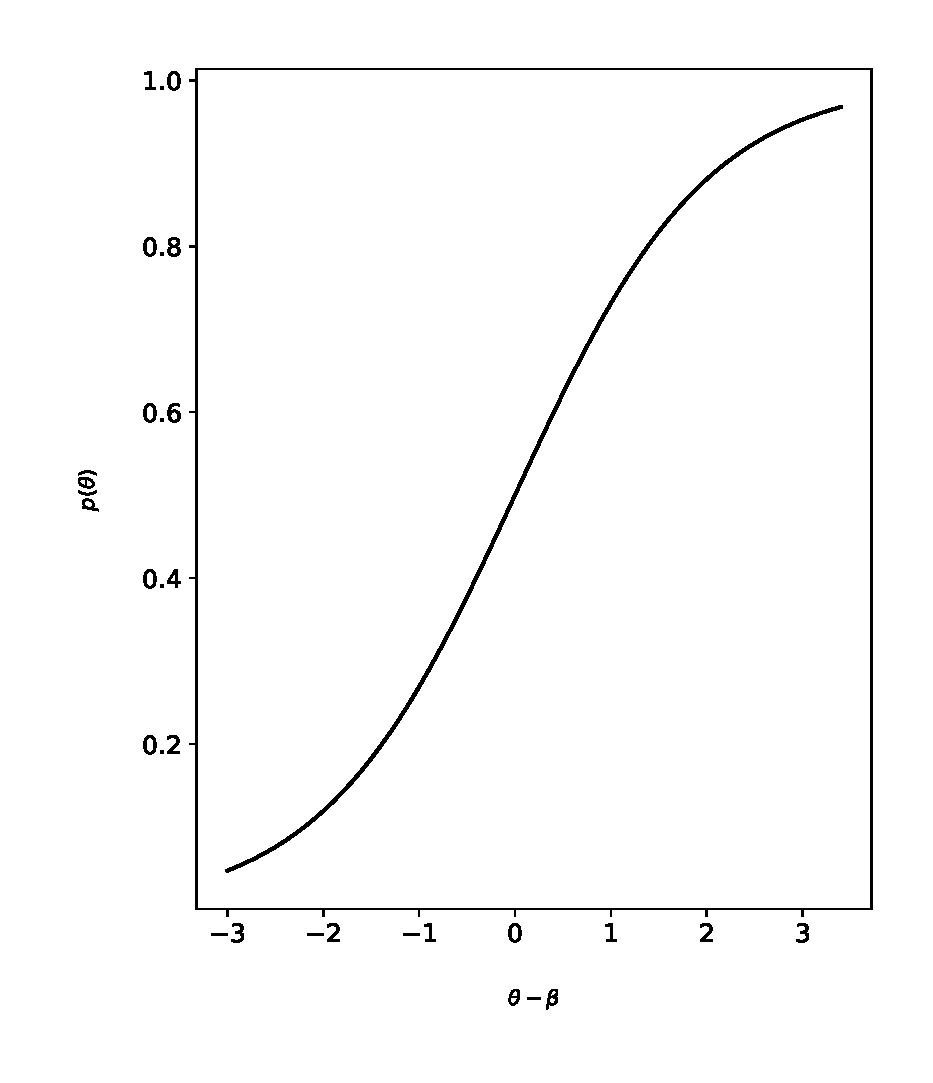
\includegraphics[width=.4\textwidth]{fig/irt.eps} 
   \caption{A probability curve in Item Response Theory.}
  \end{figure}
}



\frame{ \frametitle{Grading to Obtain Thetas}
  \begin{itemize} 
    \item We are interested in finding $\theta_s$ values for students, but
    not to grade per se (though we could). 

    \item We need them primarily in order to determine questions to ask so
    as to raise trait ability.

    \item Nonetheless, knowing how $\theta_s$ might map to grades could
    make the process more intuitive.
  \end{itemize} 
}



\frame{ \frametitle{Grade Mappings}
  \small
  \centering
  \begin{tabular}{||l|c|l||}
  \hline\hline
  Letter  & $\theta$  & Explanation \\\hline
  F  & -3.0   & unsatisfactory \\\hline
  D- & -2.5   &                \\
  D  & -2.0   & minimal        \\
  D+ & -1.5   &                \\\hline
  C- & -1.0   &                \\
  C  & -0.5   & acceptable     \\
  C+ & 0.0    &                \\\hline
  B- & 0.5    &                \\
  B  & 1.0    & good           \\
  B+ & 1.5    &                \\\hline
  A- & 2.0    &                \\
  A  & 2.5    & distinguished  \\
  A+ & 3.0    &                \\\hline\hline
  \end{tabular}
  \normalsize
}



\frame{ \frametitle{Maximum Likelihood Estimate}

  To find trait ability given a response set, define 

  \[
  f_{si}(\theta_s) =\left\{
           \begin{array}{ll}
                 p_{si}(\theta_s) & \mathrm{if}\  x_{si} = 1 \\
                 q_{si}(\theta_s) & \mathrm{otherwise}
           \end{array}
         \right.
  \]

  where 

  \[
     q_{si}(\theta_s)  = 1 - p_{si}(\theta_s).
  \]

}



\frame{ \frametitle{Maximum Likelihood Estimate}

  \begin{itemize} 

    \item That is, $f_{si}$ assumes the probability $p_{si}$ if answered
    correctly and $q_{si}$ if not answered correctly.  

    \item The probablity of observing a total response set given a particular
    $\theta_s$ value is the product of the probabilities $f_{si}$ for all $i$,
    $1 \leq i \leq n$, or

  \end{itemize} 

  \[
    \prod_{i=1}^n f_{si}(\theta_s).
  \]

}



\frame{ \frametitle{Maximum Likelihood Estimate}

  \begin{itemize} 

    \item We suppose that there exists some $\theta_s$ which maximizes this
    product.

    \item The most likely value for the student's true trait ability $\theta_s$
    is defined by:

  \end{itemize}

  \[
    \theta_s = 
    \underset{\theta}{\textrm{argmax}}
    \Bigg[ 
    \prod_{i=1}^n f_{si}(\theta).
    \Bigg]
  \]

  \begin{itemize} 

    \item That is, that value of $\theta_s$ which maximizes the product which
    gives the probability of all the observations occuring together, given
    $\theta$.  

    \item To obtain this, products for a range of possible $\theta$ values are
    calculated.

  \end{itemize} 

}



\frame{ \frametitle{Item Response Theory MLE}
  \begin{figure}[p!]
   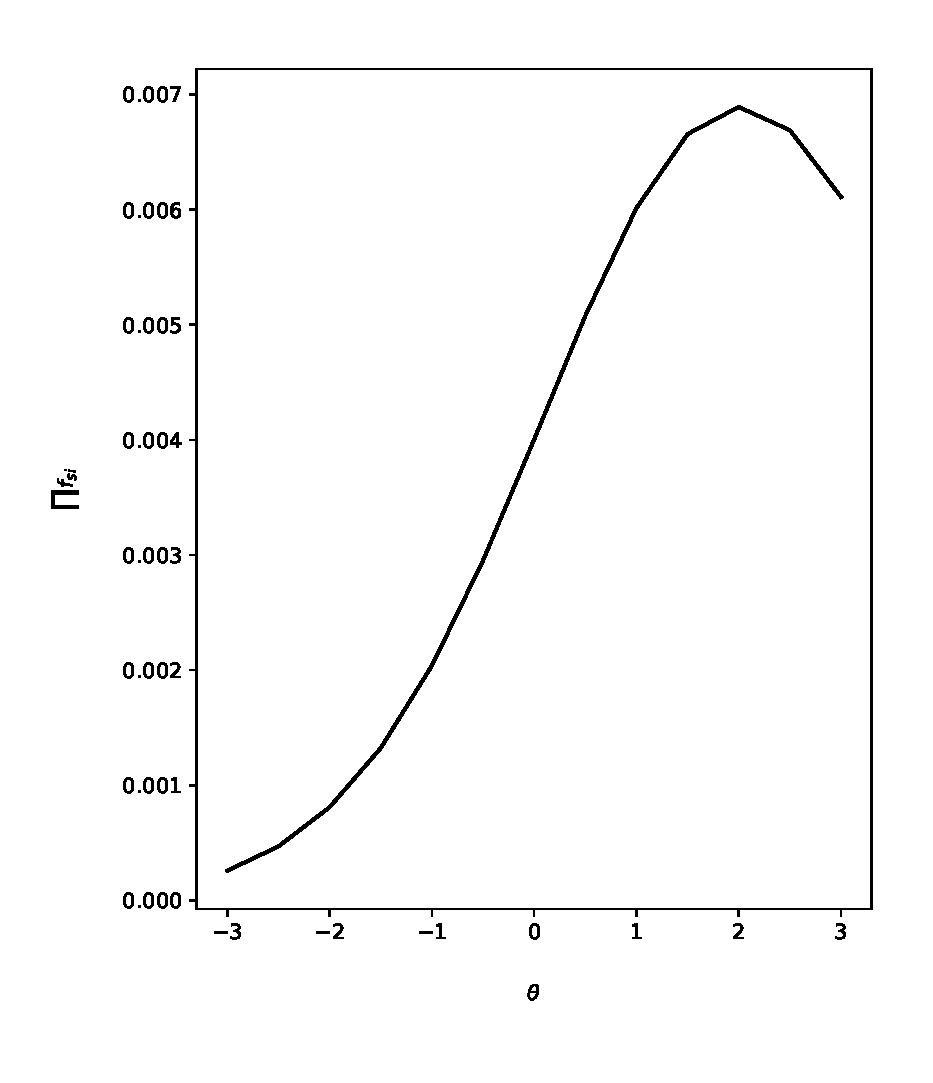
\includegraphics[width=.4\textwidth]{fig/mle.eps} 
   \caption{A maximum likelihood estimation with Item Response Theory.}
  \end{figure}
}



\subsection{Literature}


\frame{ \frametitle{ITSs and IRT}
  \begin{itemize} 

    \item One ITS/CAT uses the Rasch model (1PL model) to give a ``guided
    path'' for learners \cite{chen2005personalized}.

    \item Another uses IRT to estimate English language-learners' ability, then
    direct them to language articles of an appropriate difficulty to raise it
    \cite{yarandi2011personalised}.  Interestingly, the articles are tagged
    with difficulty.

    Another uses IRT for steps in a process-based ITS, aiming to evaluate
    every step of the problem-solving process \cite{tatsuoka1990toward}.
  \end{itemize} 

}



\frame{ \frametitle{ITSs + Bloom + IRT}

  The few ITSs which use both IRT and Bloom levels:
  
  \begin{itemize} 
  
   \item map Bloom levels to difficulty levels \cite{sitthisak}, 
   \item provide neither a clear mapping or separation of the two \cite{osborne2013grounded}, 
   \item lack a scheduler, \cite{lilley2005generation}, 
   \item or use the Rasch model \cite{ghulman2009modern}.  

  \end{itemize} 

}





\frame{ \frametitle{The Database}
  \begin{itemize}

    \item The database contains content items and assessments.  Content items
    may be informative items or questions.  
    
    \item Both have: 
    
      \begin{itemize} 
         \item Bloom level 
         \item Difficulty 
         \item Concept 
         \item Dependencies
      \end{itemize} 

    \item Questions have:
    
      \begin{itemize} 
        \item Item discriminations 
        \item Probabilities of guessing 
        \item Solutions 
      \end{itemize} 

    \item Assessments are collections of item sets, which may be represented
    as trees.

  \end{itemize} 
}







\subsection{Previous Work}


\frame{ \frametitle{Difficulty and Bloom Level}
  \begin{itemize}

    \item It is widely thought that Bloom level and difficulty are strictly
    equal \cite{newman1988effect,oliver2004course,lord2007moving,
    johnson2006bloom,fuller2007developing}. 
    
    \item Previous work \cite{castleberry2016effect} has argued the contrary,
    producing empirical evidence for the hypothesis that Bloom level and
    difficulty are separate entities.

    \item It is sufficient to find pairs of problems to serve as counterexamples:
    one at a higher Bloom level and lower difficulty than another.

  \end{itemize}
}



\section{Models and Data Structures}



\subsection{Representing Trait Ability}



\frame{ \frametitle{There are Multiple Abilities}
  \begin{itemize}

    \item A student may have differing levels of ability for different
    concepts:  good at recursion, but with pointers.

    \item For that reason, trait ability should be separated per-concept.

    \item However, a student may have different levels of ability per Bloom level.

    \item For example: 
    
      \begin{itemize} 
         \item A student may have exceptional comprehension of recursion.  
         The student can follow a recursive procedure.  
              
         \item However, the same student may have low application ability; 
         they cannot yet apply the rules of recursion to complete a 
         fill-in-the-blank code.
      \end{itemize} 
    
  \end{itemize} 
}



\frame{ \frametitle{The Trait Ability Matrix}

  \begin{itemize}
    \item Since trait ability is per-student and per-Bloom level, the
    most representative data structure is a matrix:
  \end{itemize} 

  \[
  \Theta_s =\left[
           \begin{array}{lllll}
                \theta_{s11} & \ldots       & \ldots       & \ldots & \theta_{sn1}  \\
                \vdots       & \ddots       &              &        &               \\
                \vdots       &              & \theta_{sjk} &        &               \\
                \vdots       &              &              & \ddots &               \\
                \theta_{s1m} &              &              &        & \theta_{snm}  \\
           \end{array}
         \right]
  \]
}



\frame{ \frametitle{An Example Trait Ability Matrix}
  \begin{itemize}
   \item A likely matrix may look like the following, which has a
   diagonal gradient.  
   
   \item If the course follows a progression across Bloom levels and 
   concepts, the student's ability per-concept and per-Bloom level 
   should rise accordingly over time.
  \end{itemize}
  \[
  \Theta_1 =\left[
           \begin{array}{llllll}
               3 & 2.5 & 1   & 0   & -1     & -2   \\
               2 & 1.5 & 0   & -.5 & -1.5   & -2.5 \\
               1 &  .5 & 0   & -1  & -2     & -3   \\
               1 & 0   & -.5 & -1  & -2.5   & -3   \\
           \end{array}
         \right]
  \]
}



\subsection{Representing Dependencies}


\frame{ \frametitle{Question Dependencies}

  \begin{itemize} 
    \item  Some questions have dependencies.  Consider the following; one must
    know about integer division and the modulo operations before being able to
    combine them to solve problem (3).
  \end{itemize} 

  \begin{enumerate}
   \item \emph{What is (5 \% 2)?}
   \item \emph{What is (5 / 2)?}
   \item \emph{What is (5 \% (5 / 2))?}
  \end{enumerate}

  \begin{itemize} 
    \item  It is reasonable to assume that the student's ability to handle a
    a dependency (or a dependee) influences the ability to handle the question
    which depends on the dependencies (the depender).
  \end{itemize} 

}



\frame{ \frametitle{Identifying Potential Dependencies}

  \begin{itemize}
    \item If dependencies of the form $c \rightarrow a$ and $c \rightarrow b$
    exist (that is, $c$ depends on $a$ and $b$), they may be indicated by a
    high simple matching coefficient:
  \end{itemize} 

  \[
   \frac{n_{00} + n_{11}}{n_{00} + n_{01} + n_{10} + n_{11}}
  \]

  where the values for these various $n$ are:
  
 \begin{center}
 \begin{tabular}{|l|l|l|l|}
 \hline
        &  $y=0$         &  $y=1$         &  total     \\ \hline
   $x=0$ & $n_{00}$      & $n_{01}$      & $n_{0 \bullet }$  \\ \hline
   $x=1$ & $n_{10}$      & $n_{11}$      & $n_{1 \bullet }$  \\ \hline
   total & $n_{\bullet 0}$ & $n_{\bullet 1}$ & $n$                \\ \hline
 \end{tabular}
 \end{center}


}



\frame{ \frametitle{Identifying Dependencies}

  \begin{itemize} 

    \item Alternatively, the phi coefficient, or mean square contingency
    coefficient, can be used to identify the degree of association between two
    questions.  It is defined as:

    \[
     \phi = \frac{n_{11}n_{00} - n_{01}n_{10}}
     { 
       \sqrt{ n_{\bullet 0} n_{\bullet 1} n_{0 \bullet} n_{1 \bullet} } 
     }
    \]

    \item This is the binary analogue to the Pearson correlation coefficient;
    but its range is only $[-1, 1]$ if there is a fifty-fifty split.  

  \end{itemize} 

}


\frame{ \frametitle{Assessments are Forests}
  \begin{figure}[!p]
    \centering\includegraphics[width=.6\textwidth]{fig/forest.eps}
  \caption{A forest obtained from an item set, where each tree is a subset
  of the item set which has dependency relationships}
  \end{figure}
}



\frame{ \frametitle{Some ``Dependencies'' are Not Dependencies}
  \begin{figure}[!p]
    \centering\includegraphics[width=.6\textwidth]{fig/severance.eps}
  \caption{The severance of dependency relationships based upon low $\alpha$
  values}
  \end{figure}
}



\frame{ \frametitle{The Base Graph}
  \begin{figure}[!p]
    \centering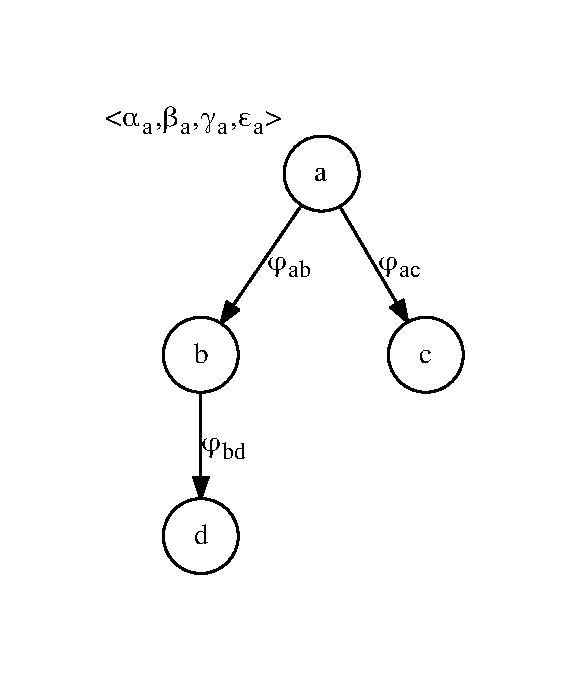
\includegraphics[width=.4\textwidth]{fig/base-graph.eps}
  \caption{The base item set graph, which includes item-specific paramters}
  \end{figure}
}



\frame{ \frametitle{The Student Graph}
  \begin{figure}[!p]
      \centering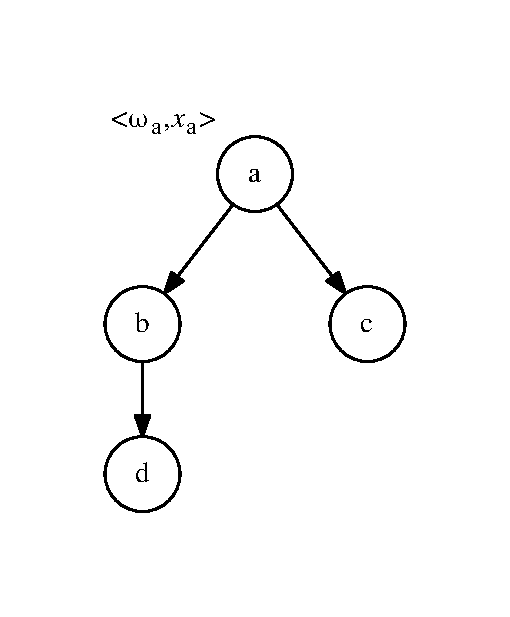
\includegraphics[width=.3\textwidth]{fig/student-graph.eps}
  \caption{The student-specific item set graph, which includes the list of
  student responses and timestamps for each response}
  \end{figure}
}



\subsection{Logistic Regression}


\frame{ \frametitle{Linear Regression}

   \begin{itemize}
     \item We might consider the use of linear regression to determine
     whether or not a student will answer a question correctly ($Y$) 
     given responses for $X_1$, $X_2$, etc.

     \item Consider the linear equation in which a binary dependent variable
     $Y$ depends on some response $X$:
   \end{itemize} 

  \[
           Y = a + bX + \epsilon
  \]

}



\frame{ \frametitle{We Shouldn't Use Linear Regression}

  \begin{itemize}

    \item Unfortunately, our particular scenario violates a few of the
    assumptions required for linear regression.  

    \item There is no linear relationship since our dependent variable is 
    categorical (0 or 1).

    \item Every linear combination of components should have a univariate 
    normal distribution, but every component only assumes one of two possible
    values.

    \item Linear regression requires homoscedasticity.  The error terms along
    the regression should be equal, but in the above situation, the variance of
    the error is dependent on the probability.   In particular
    $\mathrm{var}(\epsilon) = p(1-p)$.

  \end{itemize} 

}



\frame{ \frametitle{The Assumptions of Logistic Regression}

  \begin{itemize} 

   \item The dependent variable is binary,
   
   \item P(Y=1) is the probability that the event $Y$ occurs, 
   
   \item The model is fitted correctly, which means that there are no extraneous
   variables used in the regression, but that all variables are meaningful,

   \item That error terms should be independent; each observation should be
   independent, and little to no multicollinearity should exist.  

   \item Indepedent variables should be linearly related to the log odds of
   the event.

  \end{itemize} 

}



\frame{ \frametitle{Possible Violations}

  \begin{itemize} 

   \item The user can eliminate extraneous variables by examining $\alpha$, 
   and specifies the graph from the outset, so there \emph{shouldn't} be 
   extraneous variables.

   \item Some multicollinearity will probably exist for most dependency sets 
   due to the nature of the dependee-depender relationships.

   \item An extraction technique like PCA or factor analysis could be done to
   avoid multicollinearity. 
   
     \begin{itemize} 
       \item \ldots But then the graphs would not be as legible.  
       
       \item Plus, we would need to do PCA/FA every time the question is 
       answered, which can be expensive.
     \end{itemize} 

 \end{itemize} 

}


\frame{ \frametitle{Logistic Regression: The Formulae}

  Logistic regression is a regression of what are known as log odds. The odds
  are defined as:

  \[
    \mathrm{odds} = \frac{p}{1-p}
  \]

  And the log odds, or logit, is defined as:

  \[
    \logit = \ln(\mathrm{odds}) = \ln\Big(\frac{p}{1-p}\Big) = a + bX
  \]

}



\frame{ \frametitle{The Logistic Curve and Item Response Theory}

  Correspondingly, odds may be defined as follows:

  \[
    \frac{p}{1-p} = e^{a + bx}
  \]

  Solving this equation for $p$ yields

  \[
    p = \frac{e^{a + bx}}{1 + e^{a + bx}}
  \]

  which can be reduced to 

  \[
    p = \frac{1}{1 + e^{-(a + bx)}}
  \]

  which is called the logistic curve, which is one in the family of sigmoid
  curves.  It is identical to the type of curve used in Item Response Theory.

}


\frame{ \frametitle{The Inclusion of Dependency Information}

  \begin{itemize} 

    \item To account for item dependencies, a modified form of logistic
    regression may be sought.  
    
    \item It is desirable to keep in account the item discrimination as well as
    the trait ability of the student.  
    
    \item Here, $X_i$ is the correctness of the $i^{th}$ dependee response, and
    $Y$ is the log odds that the depender question is answered correctly:

  \end{itemize} 

  \[
    Y = b_1X_1 + b_2X_2 + \ldots + b_{n-1}X_{n-1} + b_n\alpha_i(\theta_s-\beta_i)
  \]

}



\frame{ \frametitle{A Neural Network}
  \begin{figure}[!p]
    \centering\includegraphics[width=.5\textwidth]{fig/neural.eps}
  \caption{A perceptron; a single-layer neural network, where the inputs a, b, and c
  are multiplied by weights, summed, and applied to a sigmoid squash function}
  \end{figure}
}



\frame{ \frametitle{The Dependency Graph with Weights}
  \begin{figure}[!p]
    \centering\includegraphics[width=.5\textwidth]{fig/deps.eps}
  \caption{A view of the dependency graph and weights used in the logistic regression,
  including the item parameters}
  \end{figure}
}



\subsection{Memory Models}



\frame{ \frametitle{Law of Forgetting}

  \begin{itemize} 

    \item Ebbinghaus is credited with a theory of memory and forgetting which
    has withstood empirical study for over a century \cite{ebbinghaus}, known
    as the power law of forgetting. 
    
    \item According to it, the strength of a memory after a time $t$ falls off 
    exponentially: 

  \end{itemize} 

  \[
   S(t) = ae^{-bt}
  \]

  \begin{itemize} 
    \item In this model, $a$ is the initial strength of the memory, and
    $b^{-1}$ is a decay rate.  If $a=1$, the function may be interpreted as a
    probability function:
  \end{itemize} 

  \[
   p_{recall}(t) = e^{-bt}
  \]

}



\frame{ \frametitle{The Curve of Forgetting}
  \begin{figure}[p!]
   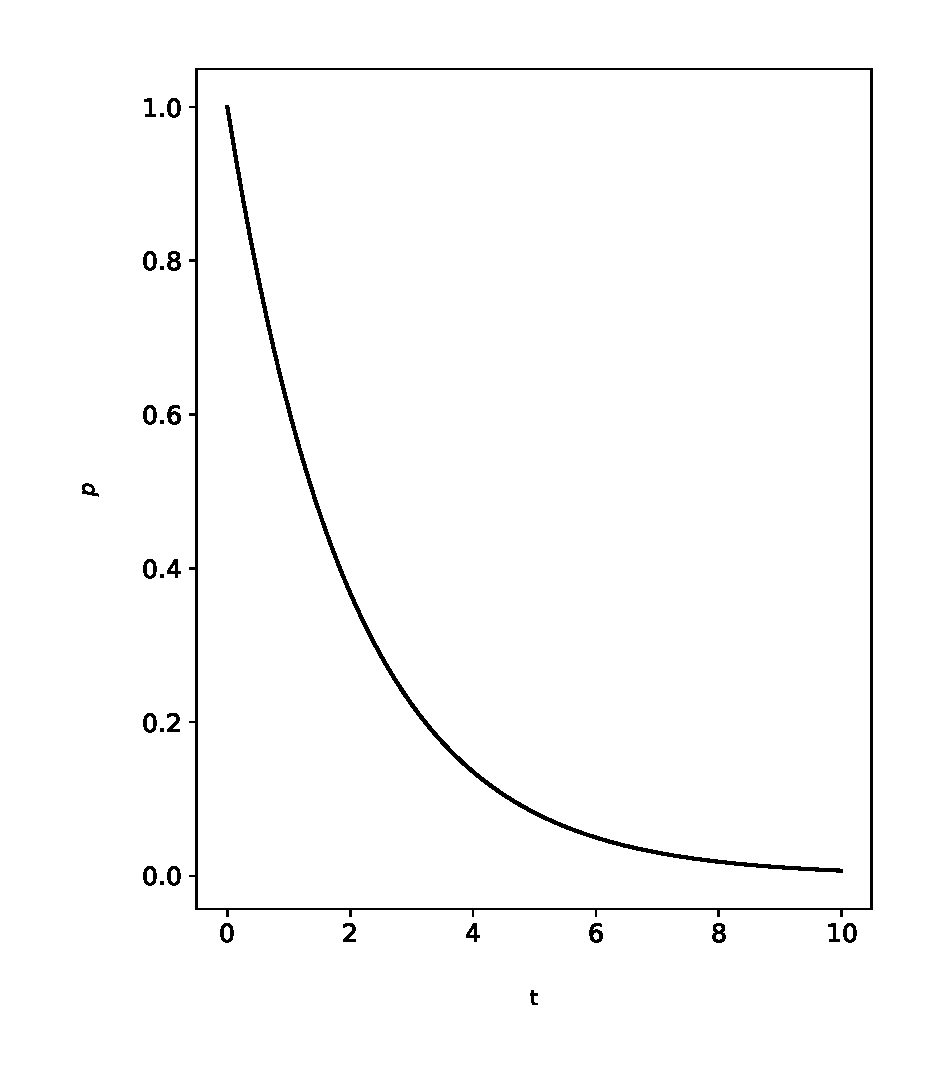
\includegraphics[width=.4\textwidth]{fig/forgetting.eps} 
   \caption{The Ebbinghaus curve of forgetting, which features an exponential
   dropoff of memory strength over time}
  \end{figure}
}



\frame{ \frametitle{The Modified Curve of Forgetting}
  \begin{figure}[p!]
   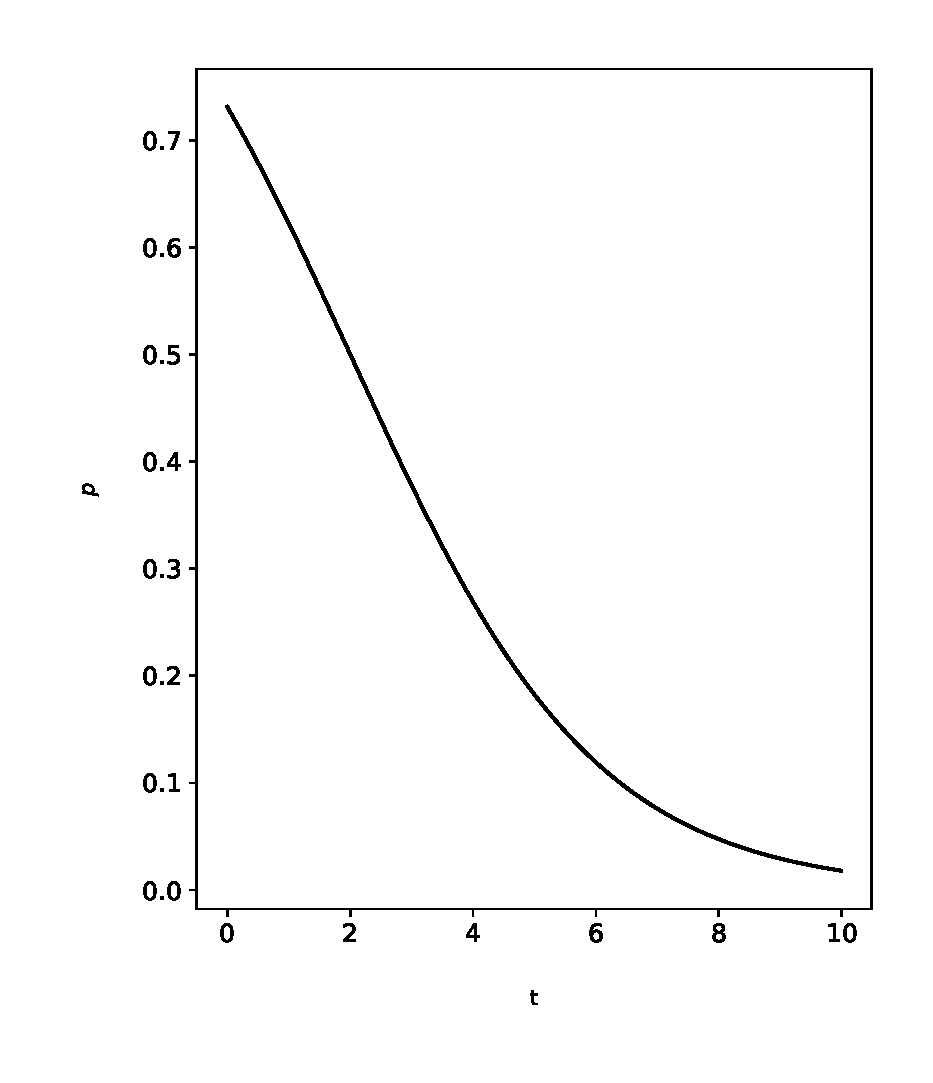
\includegraphics[width=.4\textwidth]{fig/modified.eps} 
   \caption{The modified curve of forgetting, which resembles the reverse
   sigmoid function}
  \end{figure}
}



\frame{ \frametitle{ACT-R}

  \begin{itemize} 

    \item John Anderson is credited with having developed Adaptive Control of
    Thought-Rational (ACT-R), a process-based model which simulates the solving
    of problems.  
    
    \item In ACT-R, there are goals, akin to problem statements; and rules, or
    processes used to solve problems; and finally facts, or knowledge utilized
    in the course of applying rules. 

    \item In addition to this, however, Anderson added models for memory and
    forgetting to support realistic recall probabilities and latencies, some
    of which inspire the present work.

  \end{itemize} 

}


\frame{ \frametitle{Anderson's Activation via Related Concepts}

  \begin{itemize} 
    \item According to Anderson's model, a chunk of memory $i$ is re-activated
    (or additionally activated) to the extent that other chunks of information
    (related concepts, words, ideas, etc.) which have some association to $i$
    are attended to.  
    
    \item This notion is captured in the following equation 
    \cite{anderson2000implications}:
  \end{itemize} 

  \[
    a_i = b_i + \displaystyle\sum_{i=1}^n w_j s_{ji}
  \]

}

\frame{ \frametitle{The Effect of Practice}

  \begin{itemize} 
    \item Practice has the effect of causing the base strength of the memory to
    increase, and delays cause the strength of the memory to drop off
    \cite{anderson2000implications}:  
  \end{itemize} 

  \[
    b_i = \mathrm{ln} \Bigg( \displaystyle\sum_{j=1}^n t_j^{-d} \Bigg)
  \]

  \begin{itemize} 
    \item Here, $t_j$ is the time since the jth practice of an item, and $d$ is
    a decay rate. 
  \end{itemize} 

}



\frame{ \frametitle{Forgetting with Re-Activation}
  \begin{figure}[p!]
   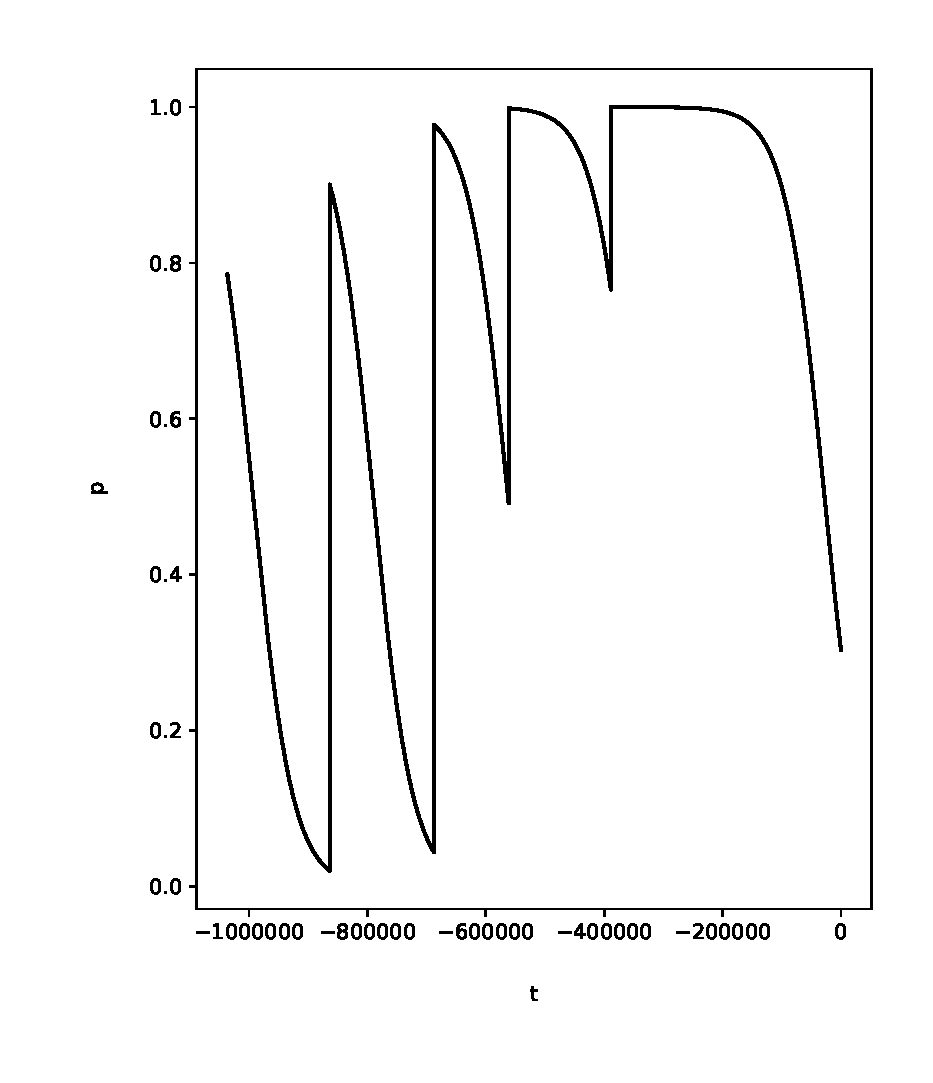
\includegraphics[width=.4\textwidth]{fig/memory.eps} 
   \caption{Forgetting with re-activation; each spike in the graph is an
   additional trial where the student is exposed to the item again}
  \end{figure}
}






\frame{ \frametitle{A Modification to the Memory Models}
  
  \begin{itemize} 
    \item A slight modification to this theory accounts for short-term memory
    and short-term memorization. 
    
    \item These allow for a small time window for the student to enjoy a high 
    probability of recollection before dropping off sharply, as in the original 
    curve:
  \end{itemize} 

  \[
    p_{recall}(t) = \frac{1}{1 + e^{{m(t-\lambda)}}}
  \]

  \begin{itemize} 
    \item In this equation, $\lambda$ is the lifespan of the memory; or, the
    amount of time that passes until there remains only a .5 probability that
    the student recalls the information.  

    \item The value $m$ is a parameter which controls the rate of dropoff, much 
    like the decay rate in Ebbinghaus' model.  
  \end{itemize} 

}



\frame{ \frametitle{Re-Activation}

  \begin{itemize} 
    \item To account for re-activation, a simple model for the extension of
    half-life may be used: 
  \end{itemize} 

  \[
   \lambda_n = \rho_s \lambda_{n-1}
  \]

  \begin{itemize} 
    \item Here, $n$ refers to exposure or trial number $n$.  In the 
    ITS, this is the nth time that the student has seen the
    problem.  
    
    \item $\lambda_{n-1}$ is the former lifespan of the memory.  $\rho_s$ is a
    learning rate, which is a parameter particular to the student; its domain
    is (1, $\infty$].  

    \item The intuition captured by this formula is that with an increased
    number of trials, the lifespan of the memory increases.
  \end{itemize} 

}



\frame{ \frametitle{Forgettability}
  \begin{itemize} 
    \item In addition, there is a difference in problems in the ease with which
    they are learned.  An addendum to this can be used to account for
    individual differences in problems: 
  \end{itemize} 

  \[
   \lambda_n = \mu_i \rho_s \lambda_{n-1}
  \]

  \begin{itemize} 
    \item Here, $\mu_i$ represents the memorability of the problem, or the ease
    with which the problem solution can be committed to memory. 
  \end{itemize} 
}



\frame{ \frametitle{The Spacing Effect}
  \begin{itemize} 
    \item The spacing effect is the effect that the amount of time in between
    trials has on the memorization of a chunk of memory.  
    
    \item In the above model, memorization is interpreted as an increase in the
    lifespan of a memory.  If only a short amount of time passes between the
    last trial, the effect will not be as great as if a longer time has passed.  
    
    \item One consequence of this is that, according to the spacing effect
    hypothesis, cramming is ineffective (where cramming is namely repeating
    trials in short bursts).

    \item The spacing effect can be accommodated in the memory model used by the
    intelligent tutoring system.  We define a function for the dropoff:
  \end{itemize} 

  \[
    \sigma_t = (1 - e^{-at})
   \]

}



\frame{ \frametitle{Forgetting with Re-Activation}
  \begin{figure}[p!]
   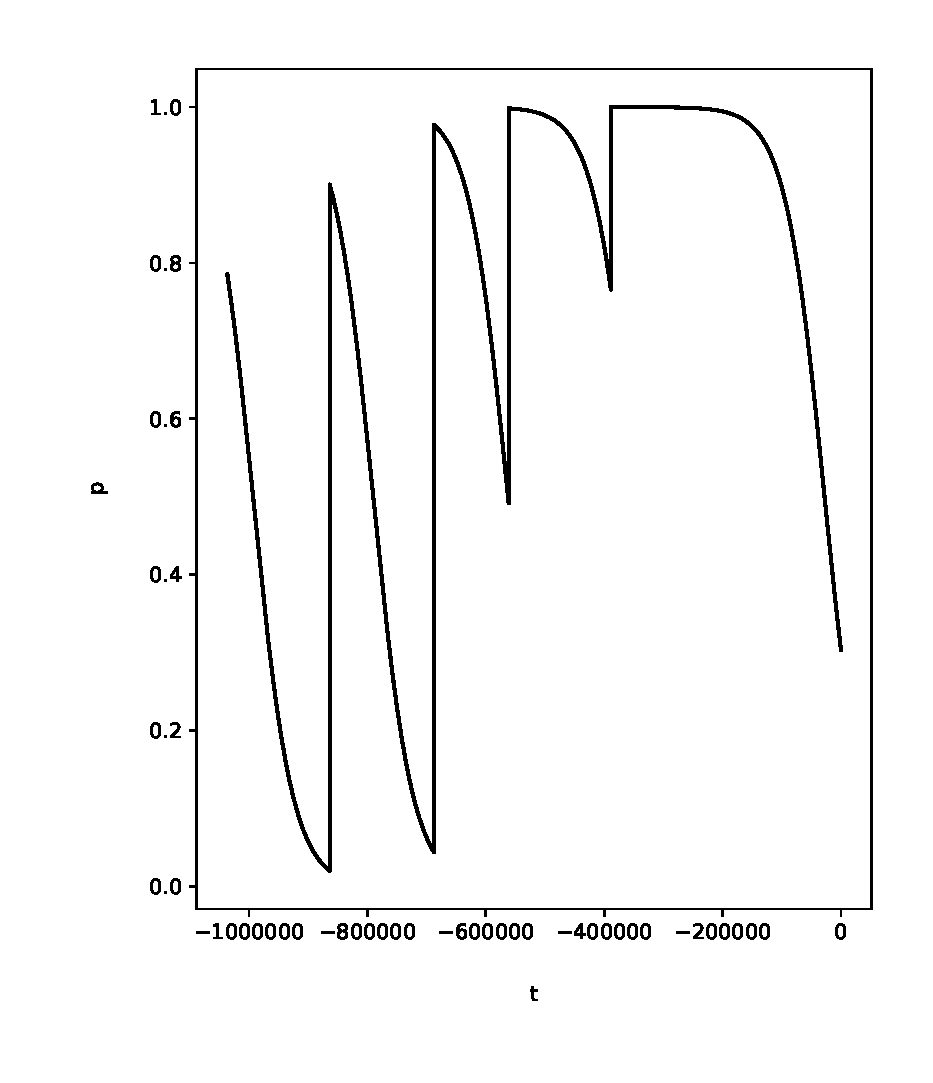
\includegraphics[width=.4\textwidth]{fig/memory.eps} 
   \caption{Forgetting with re-activation; each spike in the graph is an
   additional trial where the student is exposed to the item again}
  \end{figure}
}



\frame{ \frametitle{The Lifespans of Memories}
  \begin{itemize} 
    \item This function indicates the extent to which the spacing from the time
    the item was last seen influences the increase in the lifespan of the
    memory: 
  \end{itemize} 

  \[
   \lambda_n = (1 + \sigma_t \mu_i \rho_s) \lambda_{n-1}
  \]

  \begin{itemize} 
    \item The utility of this model is in assessing the probability with which a
    student answers a question; not only based on trait ability and dependency
    relationships, but also on the inherent tendency to forget information with
    the passage of time.
  \end{itemize} 
}



\frame{ \frametitle{Learning Curve}
  \begin{figure}[p!]
   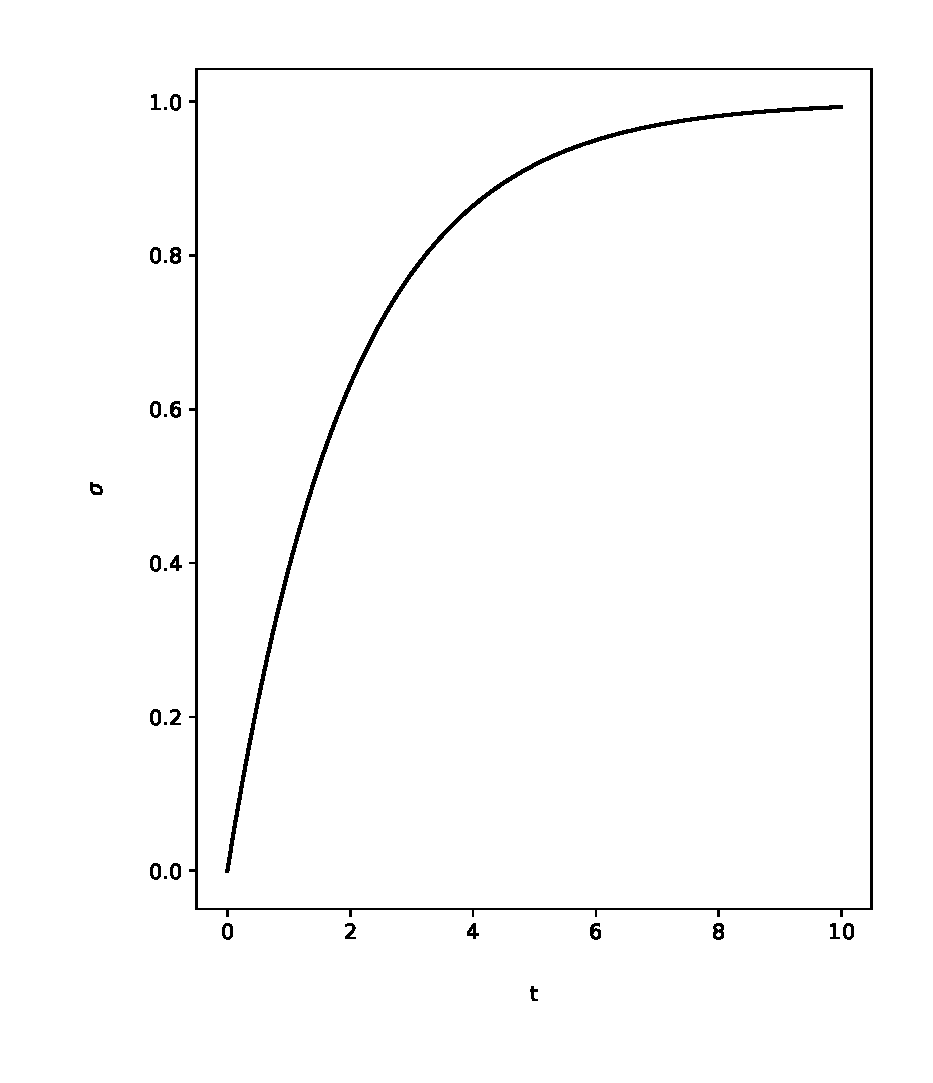
\includegraphics[width=.4\textwidth]{fig/spacing.eps} 
   \caption{The learning curve, which indicates the extent of memory
   lifespan increase given a time between trials}
  \end{figure}
}



\frame{ \frametitle{Remember or Re-Solve}
  \begin{itemize} 
  \item It will be assumed that, if a student has been exposed to a item before, then
  the probability of being able to answer the item correctly may assume one of
  two values.  

  \item The first is based upon recollection; it is the probability of
  recalling the facts, processes, and so forth required to produce the solution
  for an item.  

  \item The second is based upon derivation of the solution from known
  facts, processes, and so forth in the dependencies, as if the student were
  answering the question for the first time.  
  \end{itemize} 
}


\frame{ \frametitle{Remember or Re-Solve}

  \begin{itemize} 
    \item That is, if a student does not recall the process for solving a
    problem, the probability defaults to the probability based upon item
    parameters, trait ability and dependency relationships:
  \end{itemize} 

  \[
  p =\left\{
           \begin{array}{ll}
                 p_{recall}(t) & \mathrm{if}\  p_{recall} > p({\theta_s, x_1, \ldots}) \\
                 p({\theta_s, x_1, \ldots}) & \mathrm{otherwise}
           \end{array}
         \right.
  \]

}



\section{Algorithms for Scheduling}



\subsection{Selecting From the Matrix}


\frame{ \frametitle{Initialization}
  \begin{itemize} 
    \item First, at the very beginning of the program, the trait ability matrix
    for the student is initialized:
  \end{itemize} 

  \[
    \Theta \leftarrow -3
   \]
  
}


\frame{ \frametitle{Preliminary Testing}

  \begin{itemize} 
    \item The first iteration schedules a preliminary test consisting of a
    diagonal block of the trait ability matrix, for example:
  \end{itemize} 

  \[
  \Theta_s =\left[
           \begin{array}{llll}
                \theta_{s11} & \theta_{s21} & \theta_{s31} & \ldots \\
                \theta_{s12} & \theta_{s22} &                &        \\
                \theta_{s13} &                & \ddots          &        \\
                \vdots         &                &                 &        \\
           \end{array}
         \right]
  \]

  \begin{itemize}
    \item The test should be small enough to be feasible while having enough
    questions to support an MLE.  At least two questions are needed per (Bloom
    $\times$ concept) for an MLE. 

    \item Sometimes called \textbf{shadow testing} \cite{van2000computerized}.
  \end{itemize} 

}


\frame{ \frametitle{Question Pruning}
  \begin{itemize} 
    \item With respect to $\alpha_i$, it is desirable to discard any question $i$
    for which $\alpha_i \leq 0$.  It should be severed from the dependency tree.

    \item If $\alpha_i$ is close to -1, then the question may have predictive
    power.  

    \item With the response set, $\Theta_s$ can be constructed and the proximal
    zone of development can be identified.
  \end{itemize} 
}



\frame{ \frametitle{How to Select Categories}
  \begin{itemize}

    \item Categories with $\theta_{sjk} = 0$ are areas where the student has a
    roughly .5 probability of answering a question of difficulty $\beta=0$
    correctly.

    \item Knowing what the trait ability matrix looks like, what categories
    should be selected?

  \end{itemize} 
}



\frame{ \frametitle{Too Easy: Don't Bother}
  \begin{itemize} 

    \item The higher $\theta_{sjk}$ values should be left alone, particularly
    those nearing 3, since this demonstrates exceptional mastery of that
    category.  (Also a confidence interval can be calculated to ensure it is
    acceptable to stop.)
    
    \item In particular, if $\theta_{sjk} = 3$, there is no reason to ask
    questions from that category, since trait ability is capped at 3.

    \item As will be discussed later, there may be precedent to ask such a
    question if asking it will lead to an increase in the probability of
    answering other questions.

  \end{itemize} 
}



\frame{ \frametitle{Too Hard: The Potential for Cruelty}
  \begin{itemize} 

    \item It would be unfair (perhaps even cruel), to ask questions for which
    $\theta_{sjk}-\beta<0$; that is, those questions for which the student has
    a less than half chance of answering correctly.  
    
    \item Asking such questions consistently could have psychological
    ramifications!

    \item In the course of ordinary non-formative instruction, such questions
    may be asked, but in this case the schedule may be personalized and the
    probabilities of success are known.

  \end{itemize} 
}
 


\frame{ \frametitle{Just Right: Where p~.5}
  \begin{itemize}  

    \item The difficulty matrix for the student may be

    \[
      B_s = \Theta_s - \delta
    \]

    where $\delta$ is some (small) number.  The smaller the number, the
    harder the questions relative to the student's ability; but also the
    fewer that the student must answer to raise their trait ability estimate.

    \item Ultimately, selecting the neighborhood of difficulties to include
    questions from is a personal decision.   

  \end{itemize} 
}



\subsection{Calculations on the Forest}



\frame{ \frametitle{Initial Calculations}
  \begin{itemize} 
    \item When a student is assigned an assessment, first the probabilities that
    the student will be able to answer each question are recursively calculated.

    \item They must be calculated from the bottom-up, since internal nodes
    require probability estimates from their children.  

    \item The leaves are the only nodes that do not require logistic regression
    to obtain a probability estimate, since the leaves have no dependencies.

    \item Probability estimates for the children are obtained using Item
    Response Theory.
  \end{itemize} 
}



\frame{ \frametitle{Initial Recalls}
  \begin{itemize} 
    \item For each node which has been answered, the probability of recall can
    be calculated using the equation for recall.  
    
    \item In the presence of a probability of recall, the final probability of
    answering the question can be calculated using the combined formula.
  \end{itemize} 
}



\subsection{Seeking a Question}



\frame{ \frametitle{Finding a Question}
  \begin{itemize}
    \item Then, a recursive traversal beings at the root of each tree.  If the
    probability of answering the question at the root is within the
    neighborhood of [.5, .5+$\delta$], it is asked.  

    \item Recall that low probabilities correspond to higher differences in
    $\beta-\theta$; thus if a probability is very low, yet the student answers
    the question correctly, it will indicate a corresponding rise in trait
    ability.

    \item Such items have higher impact on the MLE estimate of trait ability.

    \item Yet if the probability is below .5, there is no reasonable assurance
    the student will be able to answer it to begin with.
  \end{itemize} 
}



\frame{ \frametitle{p Too High, p Too Low}
  \begin{itemize} 
    \item If the probability to answer the question correctly is in the
    neighborhood of (.5+$\delta$, 1],  the question is skipped.  The algorithm may
    recursively descend into its dependencies to find lower-$p$ items.

    \item If the probability is less than .5, then the system will seek to raise
    the probability by targetting the dependees, in order of the highest-impact
    dependees to the lowest-impact.
  \end{itemize} 
}



\subsection{Settling on the Dependency}



\frame{ \frametitle{Finding the Highest-Impact Dependency}

  \begin{itemize} 
    \item The dependee which controls the highest amount of variance in the parent
    probability is that dependee which has the highest coefficient in the logistic
    regression model.  

    \item However the student may already have a high probability of answering that
    dependee, such that there is little room for increases in the probability in
    the parent node due to answering the child node question correctly.

    \item Supposing $p_i$ is the probability of answering the ith dependee
    correctly, then the amount which can be gained in the dependee is:
  \end{itemize}

    \[
      \Delta_i = 1 - p_i
    \]

}



\frame{ \frametitle{Implications of 1-p}
  \begin{itemize} 

    \item If $\Delta_i$ assumes a value close to zero, it implies two things:

      \begin{itemize} 
        \item First, the student's trait ability for the dependee is high enough not to
        bother testing it, 

        \item And second, raising it to 1 would likely have little
        effect on the probability estimate of the parent. 
      \end{itemize} 

    \item Thus the highest impact item is determined not only by the coefficient,
    but also by the gain in probability for the dependee.

  \end{itemize} 
}



\frame{ \frametitle{The Odds Ratio}

  Supposing that the odds estimate for the parent $j$ were given by

  \[
    odds = e^{b_1 p_1 + b_2 p_2 + \ldots b_i p_i \ldots b_n p_n}
  \]

  Then the odds estimate for the parent $j$ if the probability were to rise
  to 1 would be

  \[
    odds = e^{b_1 p_1 + b_2 p_2 + \ldots b_i (1) \ldots b_n p_n}
  \]

}

\frame{ \frametitle{The Odds Ratio}

  Then the odds ratio would be equal to 

  \[
    \frac{ 
      e^{b_1 p_1 + b_2 p_2 + \ldots + b_i (1) + \ldots b_n p_n} 
    } {
      e^{b_1 p_1 + b_2 p_2 + \ldots + b_i p_i + \ldots b_n p_n}
    }
  \]

  which when reduced is simply

  \[
      e^{b_i \Delta_i}
  \]

}


\frame{ \frametitle{The Highest Increase in Odds Ratio}

  Thus that dependency which has the highest increase in the odds ratio is
  the item $i$ such that

  \[
    \underset{i}{\mathrm{argmax}} \Bigg[ \Big( e^{b_i} \Big)^{\Delta_i} \Bigg]
  \]

  If that dependency has a probability within the window [.5, .5+$\delta$], it is
  asked; otherwise if it has probability [0, .5), the algorithm is recursively
  applied to the dependency.

}



\frame{ \frametitle{Conclusion}
  In conclusion, we have developed a system which:
  \begin{itemize}

    \item Utilizes Bloom's taxonomy to develop a course-grained
    characterization model of student trait ability,

    \item Uses a modified form of IRT to account for dependency
    information, and

    \item Takes into account the rememberance and forgetting of 
    questions.
     
  \end{itemize} 
}



\frame{ \frametitle{Future Direction}
  \begin{itemize}
   \item More empirical validation for modified memory models,
   in particular question memorability,

   \item Downward propagation of trait ability updates through the dependency
   graph if questions are answered correctly/incorrectly,

   \item Exploring the general decay of trait ability over time.
  \end{itemize} 
}



\section{Experiments}


\subsection{Experiment 1}


\frame{ \frametitle{Experiment 1 Hypothesis}

  \begin{itemize} 

  \item The first experiment tested to see if there is a performance difference
  between computer-based assessment and paper-based assessment when questions are
  ordered by Bloom level.  

  \item The hypothesis was that students taking the computer-based assessment
  would fare better than those taking the paper-based assessment because of the
  immediate feedback offered by the computer-based assessment.

  \end{itemize} 

}


\frame{ \frametitle{Experiment 1 Design}

  \begin{itemize} 

  \item A test of 10 questions (2 concepts, each concept having questions over
  5 Bloom levels). The questions were of multiple-choice and short-answer
  format.  

  \item Participants were recruited from a Java programming course. The
  concepts were recursion and binary trees.

  \end{itemize} 

}


\frame{ \frametitle{Experiment 1 Results}

\begin{itemize} 

  \item The experimental condition ($N$=27 $M$=6.21) did in fact show a higher
  mean score than the control condition ($N$=27 $M$=5.23) in overall
  performance.

  \item Statistical significance was tested with a one-tailed two-sample
  matched-pairs Student's t-test on the composite score. The result indicated a
  statistically significant difference ($t$=2.024, $p$=0.048).  

  \item The experimental condition ($M$=4.93) showed a higher mean score than
  the control condition ($M$=4.38) in satisfaction as well; a similar t-test
  was done and was marginally statistically significant ($t$=1.7753,
  $p$=0.082).  

\end{itemize}

}



\subsection{Experiment 2}



\frame{ \frametitle{Experiment 2 Hypothesis}

  \begin{itemize} 

  \item The second experiment tested the effect of ordering the questions by
  Bloom level.  

  \item The hypothesis was that students would score better if questions were
  asked in forward Bloom order as opposed to reverse order. 

  \end{itemize} 

}


\frame{ \frametitle{Experiment 2 Design}

  \begin{itemize} 

    \item For this experiment we designed another test of 10 questions (2
    concepts, each concept having questions over 5 Bloom levels).  

    \item Participants were recruited from the same course. This test also
    covered recursion and binary trees. 

    \item In the control condition, questions were given in forward Bloom-level
    order.  In the experimental condition, they were given in reverse order.

  \end{itemize} 

}


\frame{ \frametitle{Experiment 2 Results}

  \begin{itemize} 

    \item The experimental condition ($N$=48, $M$=4.94) showed a higher mean score
    than the control condition ($N$=48, $M$=4.31).  

    \item Statistical significance was tested with a one-tailed parametric
    Student's t-test on the composite score.  The result indicated a statistically
    significant difference ($t$=2.13, $p$=0.036).

  \end{itemize}

}



\subsection{Experiment 3}


\frame{ \frametitle{Experiment 3 Hypothesis}

  \begin{itemize} 

    \item The third experiment tested the effect of intervening questions on the
    performance of later questions in the assessment.  
    
    \item Our hypothesis was that overall performance would be improved if
    incorrect answers triggered the addition of new {\em intervention} questions
    from a lower Bloom level.

  \end{itemize} 

}



\frame{ \frametitle{Experiment 3 Design}

  \begin{itemize} 

    \item The test was this time language-dependent (MATLAB) and tested mastery
    of control structures, in particular for-loops.  

    \item In the control condition, the control group was given an assessment
    of 10 questions, with 2 questions per the first five Bloom levels. The
    experimental group was given an adaptive measure.  

    \item If at any point a student answered a question incorrectly, then a
    question at the next lowest level was given.  This applied to all levels
    except knowledge.  The experimental group thus had a a maximum of 4
    additional questions asked for a total possible 14-question test.

  \end{itemize} 

}



\frame{ \frametitle{Experiment 3 Results}

  \begin{itemize} 

    \item To tell the immediate effect of the intervention questions,
    one-tailed parametric Student's t-test on the composite score of questions
    starting after the first intervention question was done. 
    
    \item It was hypothesized that the experimental condition would perform
    better on the remainder of the test. The experimental group ($N$=45,
    $M$=6.98) outperformed the control group ($N$=45, $M$=6.23).  The result
    indicated a marginally statistically significant difference ($t$=1.7082,
    $p$=0.092).

  \end{itemize}

}


\subsection{Experiment 6}


\frame{ \frametitle{Experiment 6 Hypothesis}

  For the more general form of modified IRT which takes into account
  multiple dependencies using logistic regression on the dependencies,
  we wished to test its effectiveness:

  \[
    p = \frac{1}{1 + e^{b_1X_1 + b_2X_2 + \ldots + b_{n-1}X_{n-1} + b_n\alpha_i(\theta_s-\beta_i)}}
  \]

  In our experiment to test the utility of this formula, we first required a
  small problem set with one depender and multiple dependees.  The experiment was
  intended to test whether or not the asking of highly-dependent questions
  would lead to an increase in mean scores.

}


\frame{ \frametitle{Experiment 6 Design}

  The analysis of this data required prediction on the validation set for the
  4th question.  Our hypothesis was that exposure of dependee questions should
  result in an increase in the probability that the student answers the
  depender correctly.  

}

\frame{ \frametitle{Logistic Regression Results}
  \begin{table}[p!]
  \label{tab:coeffs}
  \caption{The intercept and coefficients for the logistic regression model.}
  \vspace{12pt}
  \begin{tabularx}{\textwidth}{|X|X|X|X|X|}
  \hline \hline
                       & (Intercept)  & q1         & q2          & q3         \\ \hline
   coefficient         & -0.120870    & 0.006087   & 0.360000    & 0.407826   \\ \hline
  increase in log odds & 0.8861495    & 1.0061055  & 1.4333294   & 1.5035457  \\ \hline
  \hline \hline
  \end{tabularx}
  \vspace{24pt}
  \end{table}
}


\frame{ \frametitle{Confusion Matrix}
  \begin{table}[p!]
  \label{tab:confu}
  \caption{The confusion matrix for the logistic regression model.}
  \vspace{12pt}
  \begin{tabularx}{\textwidth}{|X|X|X|X|X|}
  \hline \hline
                       & Reference &       &     \\ \hline \hline
            Prediction & FALSE     & TRUE  &     \\ \hline
            FALSE      & 11        & 7     & 18  \\ \hline
            TRUE       & 1         & 13    & 14  \\ \hline
                       & 12        & 20    & 34  \\ \hline \hline
  \end{tabularx}
  \vspace{24pt}
  \end{table}
  }


\bibliographystyle{plain}
\frame{ \frametitle{Bibliography}
  \bibliography{mainfile.bib}
}


\end{document}
